
		\medskip
		
		Indiquer si les affirmations suivantes sont vraies ou fausses. Justifier vos réponses.
		
		\medskip
		
		\textbf{Affirmation 1 :} La solution de l'équation $5x + 4 = 2x + 17$ est un nombre entier.
		
		\vspace{3mm}
		
		\rule{\linewidth}{.5pt}
		
		\vspace{3mm}
		
		
		\textbf{Affirmation 2 : } Le triangle CDE est rectangle en C.
		
		\begin{center}
				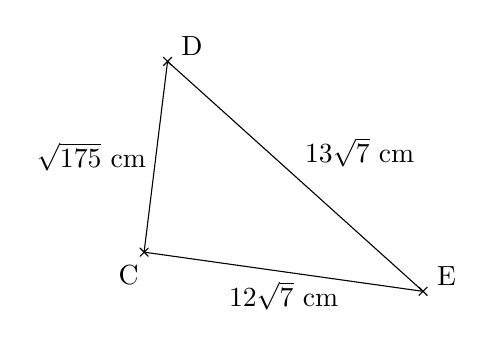
\begin{tikzpicture}[line cap=round,line join=round,x=1.0cm,y=1.0cm]
			\draw (-4.543,0.498)-- (-1.,0.) node [midway, below] {$12\sqrt{7}~\mathrm{cm}$};
			\draw (-4.543,0.498)-- (-4.245,2.920)  node [midway, left] {$\sqrt{175}~\mathrm{cm}$};
			\draw (-4.245,2.920)-- (-1.,0.) node [midway, above right] {$13\sqrt{7}~\mathrm{cm}$};
		
			\draw [color=black] (-1.,0.)-- ++(-1.5pt,-1.5pt) -- ++(3.0pt,3.0pt) ++(-3.0pt,0) -- ++(3.0pt,-3.0pt) node [above right] {E};
			\draw [color=black] (-4.542,0.498)-- ++(-1.5pt,-1.5pt) -- ++(3.0pt,3.0pt) ++(-3.0pt,0) -- ++(3.0pt,-3.0pt) node [below left ] {C};
			\draw [color=black] (-4.245,2.920)-- ++(-1.5pt,-1.5pt) -- ++(3.0pt,3.0pt) ++(-3.0pt,0) -- ++(3.0pt,-3.0pt) node [above right] {D};
			\end{tikzpicture}
		\end{center}
		
		\vspace{3mm}
		
		\rule{\linewidth}{.5pt}
		
		\vspace{3mm}
		
		\hfill
		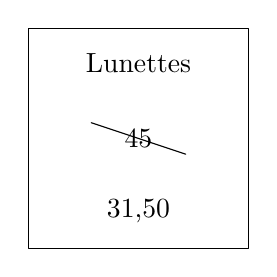
\begin{tikzpicture}[line cap=round,line join=round,x=1.0cm,y=1.0cm]
		\draw (0,0) rectangle (2.8,2.8);
		\draw (1.4,2.6) node [below] {Lunettes};
		\draw (1.4,1.4) node {45~\euro};
		\draw (0.8,1.6)--(2,1.2);
		\draw (1.4,0.2) node [above] {31,50~\euro};
		\end{tikzpicture}
		\hfill
		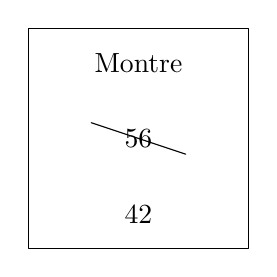
\begin{tikzpicture}[line cap=round,line join=round,x=1.0cm,y=1.0cm]
		\draw (0,0) rectangle (2.8,2.8);
		\draw (1.4,2.6) node [below] {Montre};
		\draw (1.4,1.4) node {56~\euro};
		\draw (0.8,1.6)--(2,1.2);
		\draw (1.4,0.2) node [above] {42~\euro};
		\end{tikzpicture}
		\hfill {~}
		
		\textbf{Affirmation 3 :} Manu affirme que, sur ces étiquettes, le pourcentage de réduction sur la montre est supérieur à celui pratiqué sur la paire de lunettes.
		
		\vspace{0,5cm}

